\chapter{An Introduction to Machine Learning}\label{ch:chap_2}

%
% Discuss the basics of what a machine learning algorithm is
%
In this chapter we will explain in detail the machine learning techniques used in this thesis 
including: fully-connected neural networks~\cite{Goodfellow-et-al-2016}, 
\ac{CNN}s~\cite{NIPS2012_4824} and \ac{CVAE}s \cite{1812.04405}. We will also describe 
some of the basic principals of how neural networks learn 
(i.e., backpropogation~\cite{LeCun1998}), how they are initialized, best training 
practices, methods for evaluating performance, and methods for data 
augmentation/pre-processing.

In order to dispel the notion of machine learning being uninterpretable, it should be 
stated that machine learning is perhaps most simply described as just function approximation.
The overarching goal being to approximate a function which is obtained by finding 
a global minimum according to a cost function. Although a global minimum is rarely 
obtained in reality and most often a local minimum will 
suffice~\chris{what does that mean? Surely it is a massive problem if we get stuck in a 
local minimum?}~\hunter{I would disagree with this statement.}. How one defines this 
minimised function is the key and there are many methods for doing so.

A machine learning algorithm can perform a variety of objectives 
including: classification~\cite{1404.7584}, regression~\cite{6909637}, anomaly 
detection~\cite{9243329}, denoising~\cite{1912.13171} and density 
estimation~\cite{1910.13233}. There are many other tasks a machine 
learning algorithm can tackle, but the two which are primarily used in this 
thesis are classification and density estimation. In classification, a machine learning 
algorithm attempts to learn the optimal function to classify a given set of 
inputs (e.g. a timeseries, image or any other data input) and returns as output 
the likelihood that the given input came from a particular class or set of 
classes (e.g. animal type, number). A machine learning algorithm can also alternatively 
perform non-linear regression by switching from outputting numeric values describing 
class probability to predicting a continuous variable (i.e. a changing temperature). 
Finally, we can even have a machine learning algorithm produce probability 
distributions (e.g. \ac{GW} source parameter posteriors) for a given input by 
enforcing that the algorithm predict parameters which fully describe a distribution 
% not super happy about this sentence.
such a distribution (i.e. the mean and variance of a Gaussian).

\section{Fully-Connected Deep Neural Networks}

%
% The perceptron and deep neural networks
%
So, how do we build a machine learning algorithm? Let us  
first define a simple neural network architecture, the perceptron~\cite{minsky69perceptrons}. 
A perceptron is made up of a neuron which is composed of 
several tunable variables called weights and biases. Given an input sample, 
the neuron produces a prediction on a corresponding characteristic of that 
sample (illustrated in Fig.~\ref{fig:Perceptron_network}). 
This prediction could be in the form of a class or a 
parameter value which describes that sample. Multiple perceptrons can 
then be grouped into a layer of perceptrons (henceforth referred to as neurons) 
to form a full-connected network of neurons~\cite{Goodfellow-et-al-2016}. 
Multiple layers of neurons 
can then also be stacked together to form what is known as a 
fully-connected deep neural network (illustrated in Fig.~\ref{fig:deep_nn}). 
This neural network, made up of 
many neurons, may then
trained using many samples (training samples) in order to make 
better predictions. Better predictions are achieved by adjusting the 
tunable weight and 
bias parameters of those neurons according to a term known as a cost function. 
The cost function describes how well the network
is performing with respect to the true value of each training sample~\cite{1702.05659}.

%In order to approximate 
%more complicated 
%functions, we can string together multiple perceptrons (neurons) in a layer 
%where each neuron is fully-connected to the given input $y^{m-1}_j$  
%(i.e. every element in 
%our input is multiplied by each weight of each neuron 
%in our first layer)~\cite{Goodfellow-et-al-2016}. 
%To make a deep network, we can randomly initialize another layer of neurons
%(of arbitrary size) which takes as input the output from the previous first layer %of 
%neurons (illustrated in Fig.~\ref{fig:deep_nn}). Additional 
%layers can be added in 
%perpetuity, although there are issues that can arise due to 
%a vanishing gradient or 
%hardware 
%memory limitations~\cite{1211.5063}~\chris{with this comment and the one about 
%initialisation, you are stepping ahead of the reader in terms of complexity and 
%understanding - be careful - maybe bring in these concepts when you are talking %about 
%training and backprop. I would recommend that you also add some mathematics of %how the 
%new output in a more complicated deep network depends on the nested nature of the %stacked 
%layers}. 

For the sake of simplicity 
lets presume that we want to perform what is known as a binary classification 
task, defined as having the network predict a value 
which assigns the likelihood that 
a given input belongs to one of two classes. Lets presume that the true value 
for each class is 
in the form of a number from 
0 to 1 where 0 represents one class and 1 represents the other. In order to get 
the neural network to make the correct predictions, weights and biases are 
updated according to the performance 
of the output of the network with respect to the cost function.
The cost function of a neural network can take many forms, 
but the mean squared error is one of many well established choices for a 
binary classification problem and may be defined as
%
\begin{equation}\label{eq:mean_squared_error}
    H = \frac{1}{n}\sum_{i}^{n}\sum_{j}\left(y^{M}_j(x^{(i)}) - y_{j}^{\mathrm{t}}(x^{(i)})\right)^2,
\end{equation}
%
% the loss function
%
where $y^{\mathrm{M}}_j$ is the neural network prediction from the final 
layer $M$, superscript $i$ indicates the sum over elements in 
a group (batch) of training samples ($x^{(i)}$), subscript $j$ indicates 
the sum over the output of neurons in the layer,
and $y^{\mathrm{t}}_j$ is the true class label or parameter value for 
each training sample. When 
the predicted labels over all training samples in the 
final layer $y^{\mathrm{M}}_j$ are 
similar to the training sample true labels $y^{\mathrm{t}}_i$ over 
all training samples, the cost term approaches 
zero and is near a minimum (the absolute minimum is when all predictions 
are exactly correct).

The output of each neuron in every layer may be 
defined recursively as a learned function expressed as
%
\begin{equation}\label{eq:recur_neurons}
    y^{m}_j = \sigma\left(\sum_{j}w^{m}_{j}y^{m-1}_j + b^{m}_{j}\right),
\end{equation}
%
%
%\begin{equation}
%    \Upsilon = \sum_{i=1}^{N} w_{i} x_{i} + b,
%\end{equation}
where $y^{m-1}_j$ is our given input from neuron $j$ in previous layer 
$m-1$, $w^{m}_{j}$ is our tunable scalar weight parameter, 
$b^{m}_{j}$~\chris{but $b$ 
is still just a scalar, FYI, where is $b$ in the diagram?} 
\hunter{I'm confused by what you're saying here.} is our tunable scalar 
bias term, and $\sigma$ is a non-linear function which 
rescales the output. Since we usually frame the binary classification problem such that a prediction 
of $0$ represents the first class and a prediction of $1$ 
represents the second class, we typically 
apply a sigmoid activation function (Fig. \ref{fig:sigmoid}) 
since it limits the output to be 
between $0$ and $1$. Nonlinear activation functions are 
also applied in order to allow 
our network to learn 
non-linear functions/features~\cite{1811.03378}. All weights 
and biases are typically 
initialized randomly prior to training and there are many 
schemes for choosing the 
optimal initialisation~\cite{1704.08863}.

From Eq.~\ref{eq:recur_neurons} it can be 
clearly seen that each layer is dependent on the previous layer. 
For example, 
Eq.~\ref{eq:recur_neurons} can be used to explicitly write out a 
network which has 3 layers defined as
%
\begin{equation}
    y^{3}_j = \sigma\left(\sum_{j}w^{3}_{j}\sigma\left(\sum_{k}w^{2}_{k}\sigma\left(\sum_{j}w^{1}_{s}x_s + b^{1}_{s}\right) + b^{2}_{k}\right) + b^{3}_{j}\right).
\end{equation}
where it is clear that the more layers we use, the more complex our neural 
network (expressed in Eq.~\ref{eq:recur_neurons}) becomes. 
%
%
%\begin{equation}
%    y_{\mathrm{p}} = \sigma(\Upsilon),
%\end{equation}{}
%
%
\begin{figure}
    \centering
    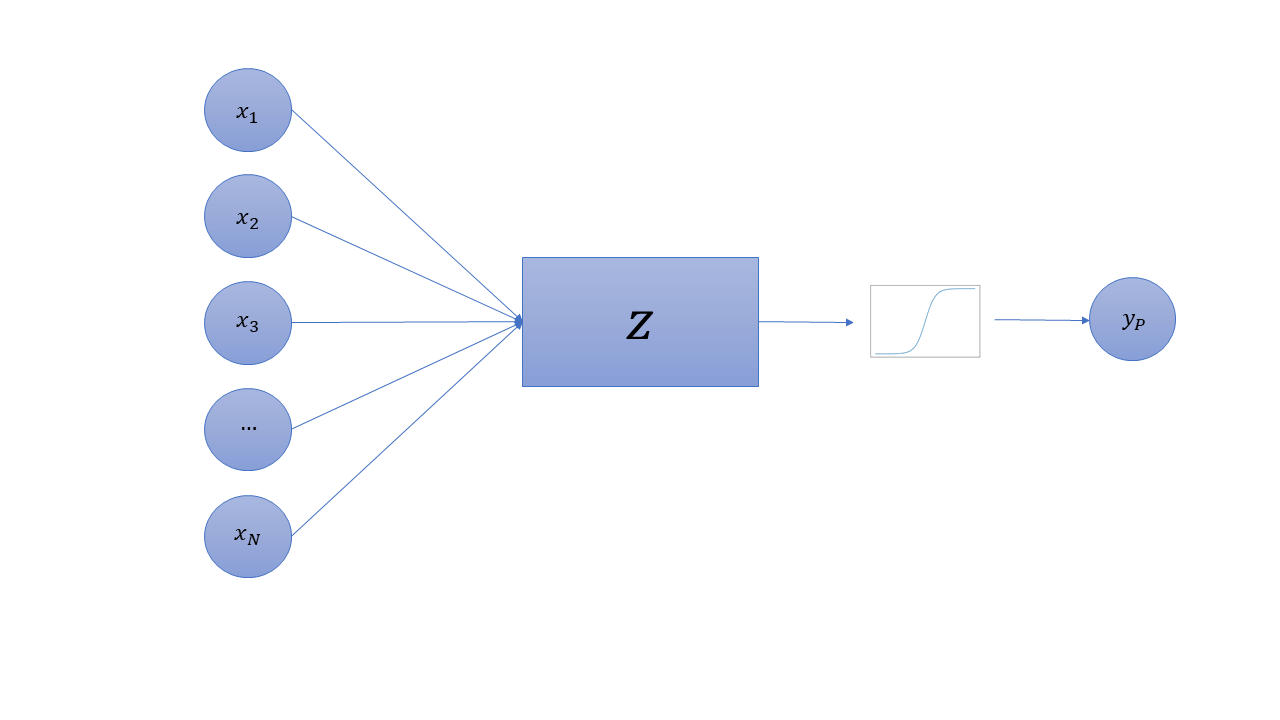
\includegraphics[width=\linewidth]{figures/Perceptron_network.png}
    \caption[Perceptron network illustration]{A perceptron network whose inputs $x_{1},\ldots, x_{N}$ are each multiplied by a learned set of corresponding weights $w_1, \ldots, w_N$ and summed together to make $z$. The summed value is then passed through an activation function to get the final output of the network, $y_{\mathrm{p}}$.~\chris{This diagram can be tidied up a bit. Where are the weights? Why is z so big and x and y are small? Why is the activation function so small and why don't you use the same sigma notation? Why does y have a p subscript?}}
    \label{fig:Perceptron_network}
\end{figure}


\begin{figure}
    \centering
    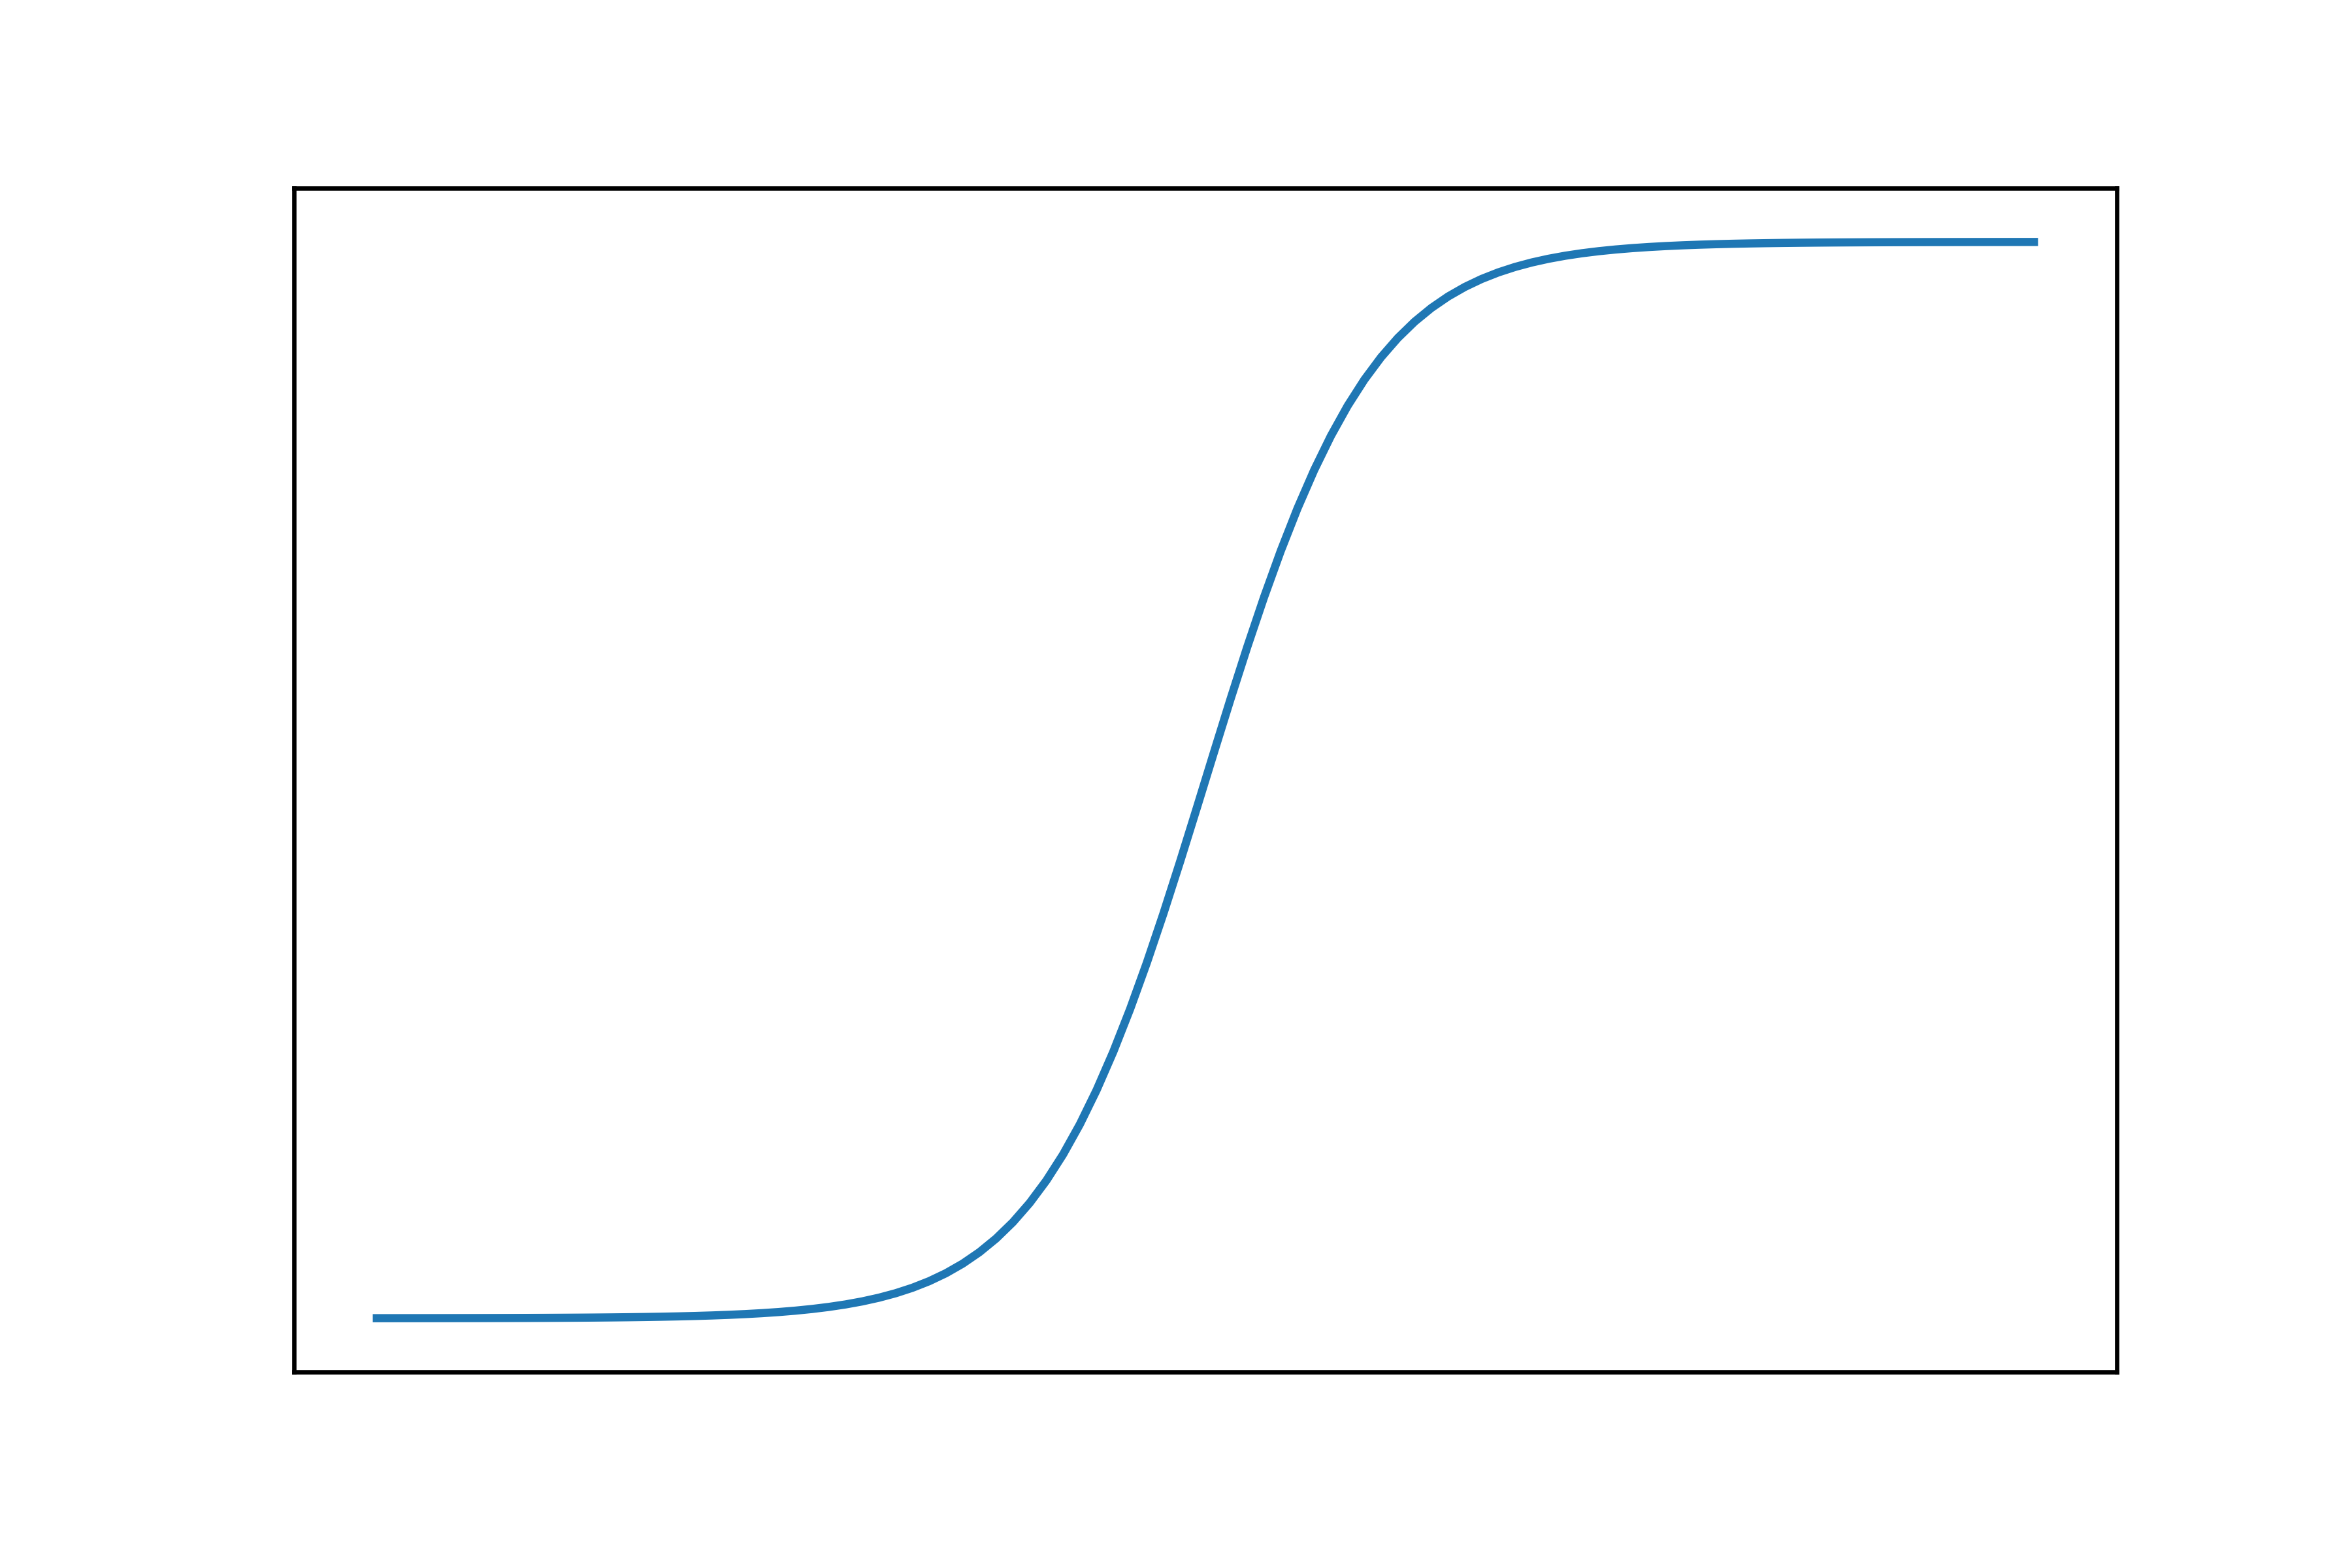
\includegraphics[width=\linewidth]{figures/sigmoid_function.png}
    \caption[Sigmoid activation function illustration.]{A sigmoid activation function plotted over the input range -10 to 10. Given an input, the activation function will rescale the input to be between the range of 0 to 1.~\chris{this is an opportunity to make the plot far more interesting and plot a whole range of common activation functions.}}
    \label{fig:sigmoid}
\end{figure}


%
\begin{figure}
    \centering
    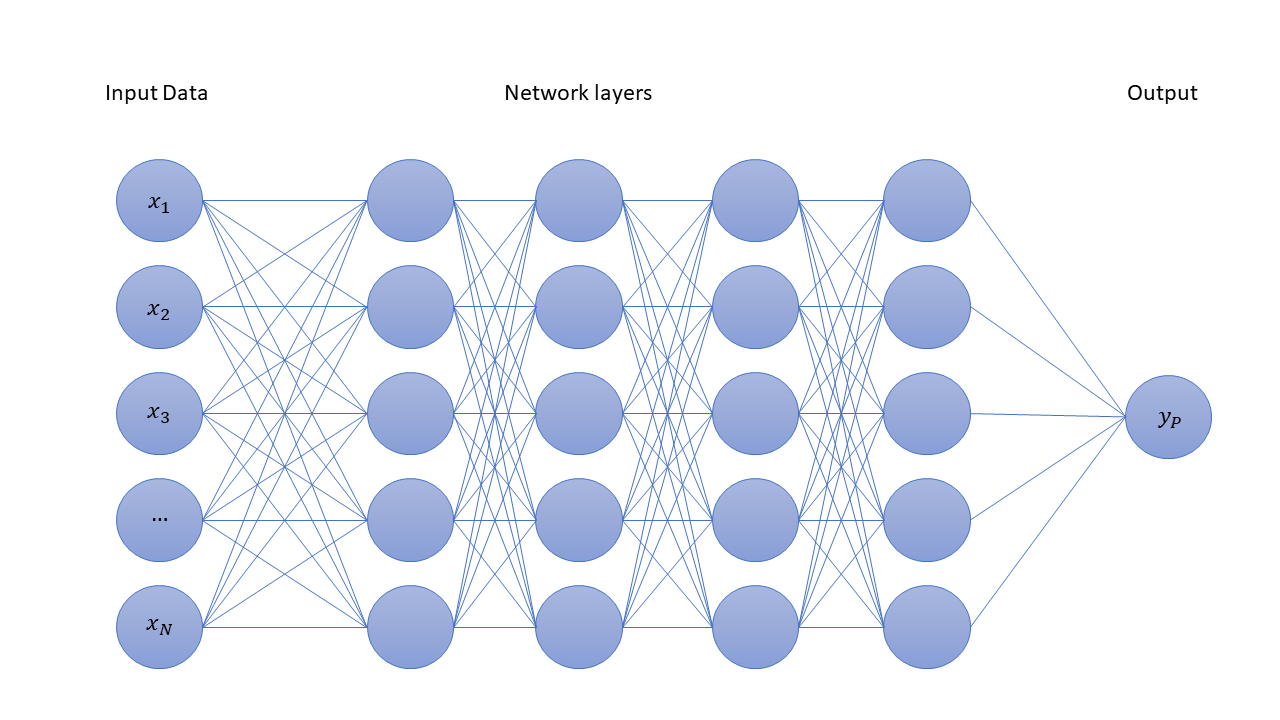
\includegraphics[width=17cm,height=20cm,keepaspectratio]{figures/DeepFullyConnectedNetwork.png}
    \caption[Deep fully-connected neural network illustration.]{A deep fully-connected neural network. Inputs $x_1 ... x_N$~\chris{sort out the latex notation} are given as input to the first layer of the neural network and are fully-connected to every node in that layer. The outputs 
    of each node are then passed on to the next set of nodes in the next layer and are also fully-connected. The final layer passes through a final single node which determines the class/value of the given input.~\chris{this diagram isn't consistent with the previous figure. There are no activation functions here, still no weights indicated, the layers are all the same size}}
    \label{fig:deep_nn}
\end{figure}
%
%\begin{equation}
%    H = \frac{1}{n} \sum_{i=1}^{n}(y^{\mathrm{p}}_i-y^{\mathrm{t}}_i)^2.
%\end{equation}{}
%

The reader's next question may 
rightly be, how does one go about choosing the right weights $w$ and biases $b$ for 
each neuron in the network? In other words, how much of an effect will 
changing $w$ and $b$ have on the resulting cost function $H$. We can quantify the amount to 
change in $w$ and $b$ such that the cost is optimised through an operation 
known as gradient 
decent~\cite{1609.04747}. We will specifically be discussing a 
variant of this optimisation method called stochastic gradient decent.

% Hebian theory "neurons that fire together, wire together"
%
% Stochastic gradient decent explanation
%
Stochastic gradient decent is an iterative algorithm used to find the global 
minimum of a function. In general, the minimum of a function may 
be determined by computing where the derivative of that function is equal to 
zero. Specifically, we are interested in minimising the cost function 
defined in Eq.~\ref{eq:mean_squared_error}. This cost function is itself 
a function the weights and biases of the neural network expressed by
Eq.~\ref{eq:recur_neurons}. \hunter{I am here in my editing.}
Gradient decent essentially has two 
decisions it needs to make when 
choosing the optimal weights and biases of a neural network: what direction to go and by how 
much~\chris{slow down! what's a direction here? All you've mentioned is changing weights and 
biases but you haven't expressed those as representing locations in a very high 
dimensionality space - within which the loss function is defined and at some 
location the loss is globally minimised}. The direction The most straightforward way of getting this 
information is through the use of a derivative, specifically the scaled gradient, with respect to network 
weights and biases,
of the cost function $H$ defined as 
%
\begin{equation}
    g = - \gamma \nabla H(y^{\mathrm{p}}),
\end{equation}{}
%
 
where $\gamma$ is a tunable step size scale factor (typically called the learning rate), 
$\nabla H(y^{\mathrm{p}})$ is the gradient of the cost with respect to the weights and biases 
of the network and $g$ is a list of scaled negative gradients corresponding to each weight and bias 
between the final output layer and the previous layer. The sign of $g$~\chris{no, the gradient is the gradient. The sign and scale are manually applied to determine which direction you want to go - and you obviously want to go downhill hence the minus sign - be clearer}~\hunter{What I'm referring to is the 
value of $g$ which can be both positive and negative for different weights and biases} for 
each weight and bias corresponds to the direction of in which to change the weights 
while the magnitude tells you how sensitive the loss function is to each weight and bias. If 
there are multiple neurons in the final layer of the network, the contributing 
gradients for each neuron in the final layer are summed in order to return a 
representative gradient with respect to all output neurons~\chris{I don't think that makes sense. Irrespective of the number of neurons in the final layer, there is one single scalar loss function. There is no summing - just a simple definition of the gradient of the loss with respect to the layer inputs.}

However, this only returns the gradients for the final output layer~\chris{well, I'm not sure about your logic here either. If you treat the input to a layer as constant then the output is only dependent on the weights and biases of that layer. So you can then write down the gradient BUT the input isn't constant if you want the gradient of the loss with respect to a weight or bias in a previous layer - hence needing back-propagation. You're right in spirit, it's just some of the terminology that sounds off.}. In  order to appropriately update weights and biases in the previous layers we must propagate the gradient backwards. This process is better known as backpropagation.

%
% Back prop explanation
%
In back propagation we use the computed gradient from the final layer and compute the 
gradient between that final layer gradient and the output from the second to last layer. 
The individual contributions from each neuron in the second to last layer are 
summed~\chris{this summing things doesn't sound right. It's pretty simple really, L 
is a function of all the weights and biases so at face value you should be able to compute 
the gradient of the loss with respect to any of the parameters. The fact that the 
output of the loss is a function of nested functions/layers means that by application of the 
chain rule you can easily obtain the gradient by multiplying the gradients between layers.} 
(same as was done in the final layer computation) and the gradients in the 
second to last layer are propagated back again to the third to last layer. Mathematically, 
we can define this process as the derivative of the loss with respect to the outputs of each layer $l$
\begin{equation}
    \nabla L(y^{l}) = \frac{\delta L}{\delta y^{(l)}}.
\end{equation}{}
~\chris{I don't know what this line is supposed to be but it looks wrong. the $nabla$ symbol implies the Del operation which returns a vector of gradients not just one gradient. Also, your derivative here is with respect to $y^{l}$ which is the output of the final layer (which could be multiple neurons).}
Applying the chain rule and expanding this out for multiple layers we arrive at
% Need to add notation describing summation over each neuron in each layer
\begin{equation}
    \nabla L(y^{l}) = \frac{\delta z^{(l-m)}}{\delta y^{(l-m-1)}} \frac{\delta y^{(l-m)}}{\delta z^{(l-m)}} ... \frac{\delta z^{(l)}}{\delta y^{(l-1)}} \frac{\delta y^{(l)}}{\delta z^{(l)}} \frac{\delta L}{\delta y^{(l)}} 
\end{equation}{}
\chris{you need to get this right and clean up the notation too. You're bringing in 
$z$ again but that only appeared in one equation and wasn't used again. 
We should probably go through this in person. It's nearly correct but not quite.} 
where the total derivative over all neurons in each layer may be quantified and 
applied to determine how much to shift each weight and bias in order to improve the 
overall loss of the neural network. This process is repeated until all weights and biases in 
the network have had their gradients computed. Ideally, we would compute the gradient 
over more than just one training sample, but rather the whole training set 
during each training iteration. However, computing the gradient over the 
whole network for all training samples is expensive, so the training set 
is typically split up into batches of samples in order to reduce the computational cost.

~\chris{As mentioned in my comments, I think the maths isn't right here. Here's a quick attempt for a super simple network. This is the loss function
%
\begin{equation}
    L = \frac{1}{n}\sum_{i}^{n}\sum_{j}\left(y^{M}_j(x^{(i)}) - y'_j(x^{(i)})\right)^2
\end{equation}
%
and the superscript $(i)$ here indicates the sum over elements of a batch, $j$ indexes over the output neurons, and $M$ is the final layer index. The prime indicates the true class label or parameter value. Every layer neuron output is defined recursively as 
%
\begin{equation}
    y^{m}_j = \sigma\left(\sum_{j}w^{m}_{j}y^{m-1}_j + b^{m}_{j}\right)
\end{equation}
%
where we've dropped the index over the input data. The upper index indicates the layer and the lower index indicates the neuron. It's easy to see that each layer depends on the previous layer. If we have 3 layers then we would have
%
\begin{equation}
    y^{3}_j = \sigma\left(\sum_{j}w^{3}_{j}\sigma\left(\sum_{k}w^{2}_{k}\sigma\left(\sum_{j}w^{1}_{s}x_s + b^{1}_{s}\right) + b^{2}_{k}\right) + b^{3}_{j}\right).
\end{equation}
%
So, you could then say that specifically for the loss derivative wrt $w^1_1$
%
\begin{equation}
    \frac{\partial L}{\partial w^1_1} = \frac{\partial L}{\partial y^{3}_1}\frac{\partial y^3_1}{\partial w^1_1} + \frac{\partial L}{\partial y^{3}_2}\frac{\partial y^3_2}{\partial w^1_1} + \ldots 
\end{equation}
%
so this is a sum over the derivatives from each output neuron, but we now need to continue expanding backwards such that the next step would be
%
\begin{equation}
    \frac{\partial L}{\partial w^1_1} = \frac{\partial L}{\partial y^{3}_1}\left(\frac{\partial y^3_1}{\partial y^2_1}\frac{\partial y^2_1}{\partial w^1_1} + \frac{\partial y^3_1}{\partial y^2_2}\frac{\partial y^2_2}{\partial w^1_1} + \ldots\right) + \frac{\partial L}{\partial y^{3}_2}\left(\frac{\partial y^3_2}{\partial y^2_1}\frac{\partial y^2_1}{\partial w^1_1} + \ldots \right.
\end{equation}
%
and so you see that you end up with this expanding sum of derivative products.
}

%
% Training best practices
%
\section{Training Best Practices (practical advice for the reader)}

I~\chris{now you start to use I instead of "we". fine but be consistent or have a consistent plan where you use I or "it" in your own chapters but "we" for the papers.} was commonly told when first wading into the pool of deep learning that the practical implementation/training of deep learning models is largely a dark art. In this section, I would like to clear up the picture by offering some best practices from personal experience when training machine learning models in general.

\subsection{Dataset Size, Pre-Processing and Augmentation}

%
% When in doubt, make more training data
%
\subsubsection{Training Data Size}
%
When in doubt, the more training data you make available to yourself, 
the better~\cite{2019arXiv190110496L,2021arXiv210209382K}. Time and again, during a large part of this thesis work, we~\chris{again, be consistent I or we?} would spend countless hours tuning and tweaking the neural network architecture only to run up against some insurmountable~\chris{was it insurmountable, maybe seemingly insurmountable since you did surmount it in the end} wall of impeded progress. Only then to increase the number of training samples by several factors and see a significant increase in performance. There is no hard rule for the exact number of training samples 
needed, as it is dependent on many factors associated with the problem being addressed, including: the structure of the data, the data space itself~\chris{using a colon to make a list and then only having 2 items in the list?}. There is some theoretical work using the concept of \ac{VC} Dimension~\cite{inbook} which may possibly inform the practitioner on a lower bound for the number of training samples to use (typically of order billions of training samples for a standard fully-connected network~\cite{inbook}). However, it should be noted that this concept is only applicable to a handful of standard algorithms and there is much disagreement in the computational science literature concerning the relevance of VC~\chris{use the acronym package} dimension in the practical implementation of machine learning 
algorithms~\cite{2017JSP...168.1223L,2016arXiv161103530Z,2018arXiv180303635F}. Specifically, it is known that simple neural network models perform well using a lower number of training samples than the VC~\chris{use acronym package} dimension would demand.~\chris{interesting stuff - new to me so I can't comment on the details. Make sure that you would be happy being questioned on this VC concept in a viva.}

\subsubsection{Data pre-processing}
%
Commonly, input datasets may span a large \chris{dynamic?} range of several orders of magnitude. In order to help the network learn more efficiently, it is beneficial to perform some pre-procesing steps~\cite{589532}. It's important to do this because if our~\chris{the?} input data has large values over a wide range, and our network is trying to learn a mapping from input to prediction, the learned weights may also end up being very large. Large learned variable weights can lead to large gradients which cause the network to update weights in large step sizes, making the whole network more unstable in the process. Normalisation can also help ensure equal importance is assigned to all features in the training set~\cite{SINGH2020105524}, i.e., greater numeric features do not dominate smaller numeric features. We~\chris{be consistent} can partially solve this issue by normalising our~\chris{be consistent} input dataset~\chris{check that you are using dataset, data set, or data-set consistently} to be between the range of zero to one~\chris{.For example, - remember that equations are part of the flow of the text so they are part of the sentence and can't just stop talking and stick in an equation. Also, the normalisation doesn't need to be betyween 0 and 1, in fact, we use -1 and 1 and in the CNN paper we didn't restrict the range. Maybe make it clear that there are multiple options.} 
\begin{equation}
    y = \frac{x - x_{\textrm{min}}}{x_{\textrm{max}}-x_{\textrm{min}}},
\end{equation}
where $y$ is our new normalised data, $x$ is our original unnormalised~\chris{you might need a hyphen?} data, $x_{\textrm{min}}$ is our unnormalised data minimum value and $x_{\textrm{max}}$ is our unnormalised data maximum value. It can also be advantageous to rescale our~\chris{be consistent} input data to a standard normal distribution if our data has widely varying scales by applying 
\begin{equation}
    y = \frac{x - x_{\textrm{mean}}}{x_{\textrm{std}}},
\end{equation}
where $x_{\textrm{mean}}$ is the mean of our data and $x_{\textrm{std}}$ is the standard devitation~\chris{the standard notation would be $\sigma_{x}$} of our data. In addition to rescaling our input data, we occasionally need to also rescale our training labels. This is especially relevant if the activation function in our final neural network layer is fixed to be between some values. For example, if we were using a sigmoid activation function where the values of the output of the sigmoid are only allowed to be between zero and one, then we would also want our training label values to lie between zero and one since the network would not be able to produce values outside of that range.~\chris{I increasingly see output layers for regression not using any activation for this reason. In any case rescaling things to O(1) is always sensible.}

\subsubsection{Data Augmentation}

Neural networks can sometimes be composed of hundreds, thousands, even million of parameters to be tuned during training. Given the massive number of parameters, many complex networks require an equally massive number of training samples. But, what do you do if you are only given a limited number of training samples? This is where data augmentation comes to the rescue. In order to generate more training data, we can apply simple shifts to the existing limited dataset and greatly expand the number of training samples. Data augmentation can be accomplished in various ways, including the methods briefly 
mentioned here:

\begin{itemize}
    \item Translation: Shifting the input data sample across $n$ dimensions in the input data sample space.
    \item Rotation: Rotate data about a fixed point.
    \item Cropping: Choose a random subset of the input sample, remove all data outside of subsection, rescale cropped data to original input size.
    \item Gaussian noise: Add varying amounts of Gaussian noise in order to simulate poor quality signals.
\end{itemize}

%
% The purpose of Validation
%
\subsection{Validation}
In order to understand how well your model is performing with respect to the training data, one may plot the resultant average output of the loss function as a function of the number of training iterations. Ideally, we would like the loss to rapidly decrease and to then flatten out. Although this will give us an indication of how well the network is performing on the training set, it does not inform us as to how well the model will generalize to a novel testing set. In order to quantify the generalization ability of the network, we may set aside a small portion of the training set prior to training as a validation set. During training, we can temporarily fix the weights and run the validation set through the model in order to compute a validation loss. 

If we plot both the validation loss and the training loss as a function of time, we again ideally would like to see both curves decrease as a function of training iteration and then level out. However, if we see that the training curve initially decreases and then continues to decrease while the validation curve initially decreases and then subsequently increases we may say that the model has overfit the training data. Overfitting the training set generally indicates that either our model is too complicated and has essentially memorized the training set or that we do not have enough training data to sufficiently cover the entire parameter space. Overfitting can be mitigated by increasing the training set size, adding dropout connections (see Regularization sub section), early stopping of the training run or reducing the complexity of the neural network.

If on the other hand we see that the validation loss decreases far quicker than the training loss then we may say that the model has underfit the data, which is generally an indication that the model needs to have an increased capacity.

%
% Regularization techniques
%
\subsection{Regularization}\label{sec:ml_regularization}

%
% Dropout
%
Regularization is used to help prevent a machine learning model from overfitting the the training data. One of the easiest regularization techniques to implement is \textit{dropout}. Dropout may be implemented across most types of neural network layers (i.e. fully-connected, convolutional filters, etc.) and rarely have any adverse effect on training. During training, if dropout is implemented a randomly selected 
subset of the neurons in a layer will be switched off and not used when the gradient is computed and backpropogated through the network for a given training iteration. The percentage of neurons in a layer to switch off is a tunable parameter, though typically it is best to set a value of no more than $50\%$. Dropout effectively forces the neurons in a dropout layer to be able to identify multiple features, rather than to focus a small subset.

%
% Batch noramlization
%
Batch normalization aims to reduce the space over which the neural network has to search. As such, 
batch normalization is essentially a normalization of the output of individual layers within a neural network to be between zero and one. This normalization prevents weights or biases from becoming too large. It is computed by normalization of the current layer according to the mean and standard deviation of the output of the previous layer and the subsequent rescaling through two learned variables ($\alpha$ and $\beta$) and is formalised as 
\begin{equation}
    z_n = \alpha \hat{z}_n + \beta,
\end{equation}{}
where $\alpha$ is a learnable parameter, $\beta$ is a learnable parameter and $\hat{z}_n$ is calculated by 
\begin{equation}\label{eq:batch_norm}
    \hat{z}_n = \frac{1}{n} \sum_{i=1}^{n} \frac{z_n - \mu}{\sigma^{2} + \epsilon},
\end{equation}{}
where $z_n$ is the output of the neural network layer summed over all outputs in the batch of that layer, $[\mu,\sigma]$ are the mean and standard deviation respectively of the batch of previous layer outputs introduced to the network and $\epsilon$ is a small constant. If it turns out that the application of batch normalization is not optimal, then the network may undo the above normalization in Eq. \ref{eq:batch_norm} through the optimization of $[\alpha,\beta]$ in each layer.

\subsection{Hyperparameter Optimization}\label{sec:hyperpar_optim}
Given the increased complexity and time cost of training neural networks 
in recent years, choosing the optimal settings (hyperparameters) for a given 
model is key to efficient resource/time management. For example, for a 
practitioner trying to train a standard model such as ResNet-101~\cite{2015arXiv151203385H}, 
training the 
model to completion can take $O(24)$ hours and further tuning of hyperparameters to 
find the optimal ResNet-101 model can take several weeks~\cite{2018arXiv180705118L}. Hyperparameters 
may govern a number of model attributes, as well as model performance and may include: 
the number of neurons, number of layers, 
learning rate, activation function, etc.  
In this section, I will 
describe three approaches that have been either used or tried during the 
course of this thesis work to optimize hyperparameter choices for a given model.

\subsubsection{Random Search}
Probably the simplest of the three approaches random search 
seeks to choose model hyperparameters given a 
predefined prior distribution for each hyperparameter. 
The user may define whatever distribution they prefer 
whether that be a multivariate Gaussian distribution 
or a uniform distribution and may also choose the 
bounds of that distribution. Optimisation is carried out 
in a series of trials, whereby a random subset of hyperparameters 
is sampled from each hyperparameter distribution and the model 
is trained for a number of training iterations determined beforehand 
by the practitioner. Since by definition 
a random search is sampling statistically 
independent hyperparameter realisations from a 
distribution, one gains some practical benefits 
from this statistical independence. One of those benefits being the 
fact that the optimisation process may be stopped at any time 
for the aggregate trials to form a complete experiment~\cite{JMLR:v13:bergstra12a}. 
Additionally, if a trial fails (i.e. computing cluster shuts down 
expectantly), the trial may either be restarted or discarded completely 
without having any affect on the statistical significance of the 
aggregate trials performed~\cite{JMLR:v13:bergstra12a}.


\subsubsection{Grid Search}

In a grid search approach we define both an upper and a lower limit 
for each hyperparameter. Additionally, we define a step 
size by which we will increase the the hyperparameter 
value after each model evaluation (much like steps 
on a ladder). Each of these hyperparameter 
ladders are iterated over in an $n$ dimensional grid, 
where $n$ is representative of $n$ hyperparameters 
describing the model. Although a coarse spacing 
in $n$ dimensional grid may make it likely that the 
practictioner is sufficiently sampling the hyperparameter 
space, grid search suffers from the curse of dimensionality, 
whereby as the number of hyperparameters used (dimensions) 
increases, the number of evaluations required to perform 
trials across the entire grid increases exponentially~\cite{JMLR:v13:bergstra12a}.

\subsubsection{Gaussian Process Bayesian Hyperparameter Optimization}

Bayesian hyperparamter optimization aims to minimize (or maximize) some 
objective function. In this case, we aim to learn an 
approximate surrogate model for an objective function which 
describes the loss function space and to minimize the value of the 
loss function output. The dimensionality of the search space 
is parameterized by the number of neural network hyperparameters being optimized 
and does not usually perform well past 20 dimensions. Gaussian process 
regression is used in order to minimize the uncertainty on the surrogate model estimate 
. We then use an acquisition function to sample from the approximate 
surrogate model to determine the next set of hyperparameters to use 
during the next round of neural network training \cite{1807.02811}.

In practice, we first choose an initial set of hyperparameters 
to use in order to train the network. This can either be randomly chosen 
from a reasonable prior, or a best guess from the practitioner. 
Next, the neural network is trained a pre-defined number of 
training iterations and the network loss function output value 
is given as input to the Bayesian optimization algorithm. The Bayesian 
optimization algorithm then updates its surrogate model 
based off of this new loss value from the neural network 
given the hyperparameters used and a new set of 
hyperparameters is chosen by an acquisition function based 
informed by the Gaussian process regression surrogate model. 
The above process is repeated for $n$ user pre-defined iterations.
%
% Note, fill out this section using the following resources:
% https://arxiv.org/pdf/1807.02811.pdf
% https://towardsdatascience.com/tl-dr-gaussian-process-bayesian-optimization-5e66a014b693

\section{Convolutional Neural Networks}

\ac{CNN}s were first made popular in the late 1980s to early 1990s 
and one of the most famous examples is that of the LeNet archetecture 
made by Yann LeCunn in 1998 \cite{726791}. In his paper, LeCunn 
illustrated that \ac{CNN}s outperformed other simpler 
techniques like K Nearest Neighbor and fully-connected 
neural networks on a variety of image recognition 
tasks. In recent years \ac{CNN}s have been applied to 
many more domains including image object detection, 
fraud identification, healthcare analysis and many 
others. In this section I will explain how \ac{CNN}s work, 
mechanisms for improving \ac{CNN} performance, and 
why they are so powerful for image based tasks.

\subsection{The Convolutional Filter}

% 
% Really need to rewrite section about odd filters ...
% 
The basic building block of a \ac{CNN}, convolutional 
filters, are analogous to neurons in a standard fully-connected 
neural network. A convolutional filter is typically made up of 
an $N \times N$ matrix ( for illustrated 
example, see Fig.\ref{fig:cnn_filter_illustration}). Normally, 
the dimensions are of odd size because all pixels from the input 
to the filter are enforced to be centered around the output 
of the filter. This effectively acts to anchor the output 
of the filter, in a sense acting to interpolate all 
the anchor pixels neighboring pixels. Without using odd size filters, distortions 
across multiple layers can cause issues, though such issues can be overcome through 
added network complexity.

\begin{figure}
    \centering
    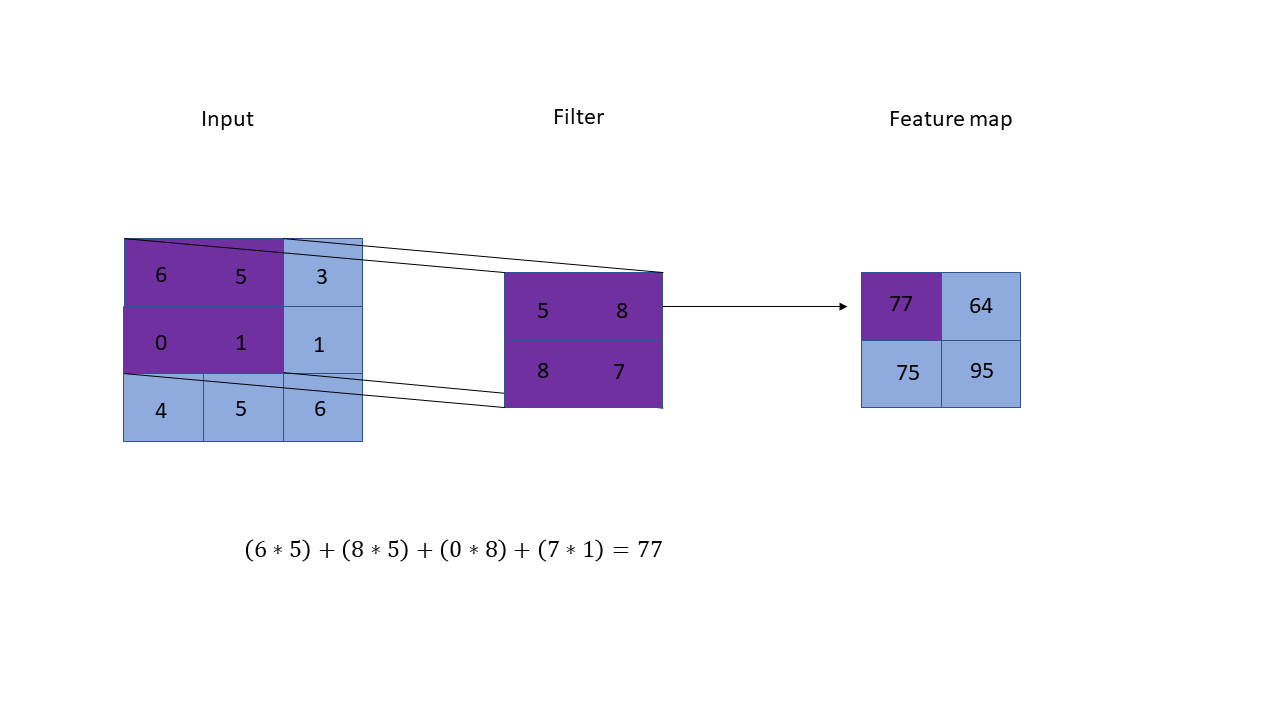
\includegraphics[width=17cm,height=20cm,keepaspectratio]{figures/cnn_filter_illustration.png}
    \caption[Convolutional neural network filter illustration.]{An illustration of a simple \ac{CNN} filter. The filter is a $2 \times 2$ filter randomly initalised with a set of weights for each dimension. Each filter weight is multiplied by the corresponding input dimension over which it is currently covering. All multiplied values are then summed together to produce the output of the filter. The filter slides over one element (if stride is set to 1) and the computation is done again until the whole input space has been covered.}
    \label{fig:cnn_filter_illustration}
\end{figure}

Values in the $N \times N$ matrix of the filter are initialised 
randomly with an added bias term. The initialised values in the 
filter are the weights of the filter. During training, the filter is 
convolved with its given input where each element in the filter 
is multiplied by the corresponding overlapping element in the 
input. All the multiplied values are then summed together to produce 
the output of the filter. A bias term is then added to the 
output. We then slide the filter over by 1 column and repeat 
the convolution process until the edge of the filter reaches 
the last column of the input. We then slide the filter back to 
the 1st column of the input and down one row and repeat 
the convolution process on all columns again. This is done 
until we have convolved the filter over the whole input.

\subsection{Pooling Layers}
Pooling is a form of regularization and acts to choose 
the most important features in each convolution of a filter. 
We do this because \ac{CNN} filters will often focus 
on minute detailed information, but lose sight of the 
bigger picture. This means that small changes in the 
input, will have large effects on the filter. In order to 
combat this, pooling acts to downsample the input, making 
it more ``fuzzy'' in the process, forcing the model 
to learn broader features.
This is done by taking the maximum value over all elements 
after a convolution and discarding all other values. 

\subsection{Striding}
In addition to pooling, another form of regularization is 
striding. Striding determines the number of pixels a 
convolutional filter moves after each convolution 
is performed. Standard techniques which use striding 
nominally employ 
a stride of 2. The two main reasons why striding is applied 
are to reduce the spacial complexity from one layer to the 
next and to reduce the overlap of the receptive field\footnote{
Receptive field is defined as a region of the input 
space to a given layer which affects the output of the 
filter being used.} 
of the \ac{CNN}~\cite{2017arXiv171202502K}. With regards to 
spacial complexity reduction, 
because we are skipping over some parts of the input when 
sequentially sliding the filter from column to columna and 
row to row, we reduce the amount of computations 
required and thus the total memory usage of a 
\ac{CNN} during training. In terms of reducing overlap 
of the receptive field, if we reference Fig.~\ref{fig:cnn_filter_illustration}, 
and imagine the input grid to be a $4\times4$ grid,
we can see that with a stride of unity (one) from left to right, 
the pixels in the corners of the of the input will only 
be convolved with the filter once, whereas the two pixels in the middle 
will each be convolved twice. With a stride of two both the middle 2 
and outer 2 pixels will only be convolved once, thus reducing 
the amount of repeated convolutions of a filter over some of 
the receptive field and giving more equal importance 
to all areas of the input space. 

\subsection{The Fully-Connected Layers}
Following the convolutional filter layers, we now 
have to convert the output of the CNN to predict 
a discrete set of classes or regress on some parameter. 
If performing binary classification, one could simply 
make the last layer of the \ac{CNN} two 1D convolutional 
filters, however this is usually not what is normally 
done. Typically, a flattening operation is applied 
to the last convolutional layer where the concatenated 
feature maps from the previous layer's filters 
are flattened into a 1D string of elements. This 1D 
string of elements are then given as input to 
a fully-connected layer of neurons. One can then add 
additional fully-connected layers and a final 
layer equivalent to either the number of classes to 
predict, or the number of parameters to regress on. 
A logical question may be why add this extra 
fully-connected complication? The primary reason 
for the addition of fully-connected layers is that we want 
to unify the learned features across all 
\ac{CNN} filters and use those features as a unified 
whole to learn how to either classify or regress.


\section{Conditional Variational Autoencoders}\label{sec:cvae_intro}

In this section I will describe the network architecture of a 
\ac{CVAE}. This will be done by first describing an \ac{AE} network, then 
a \ac{VAE} network and finally a \ac{CVAE} network.

%
% Autoencoders
%
\subsection{Autoencoders}

An \ac{AE} is 
comprised of two neural networks called an 
encoder and decoder. The encoder is given an input 
from a pre-generated training set (in this case, lets assume 
we are dealing with the MNIST dataset~\cite{lecun-mnisthandwrittendigit-2010}
\footnote{The MNIST dataset is a large database of handwritten 
digitised images written by both National Institute of Standards and 
Technology employees and student volunteers. The set is subdivided into 
60,000 training images and 10,000 testing images. Each image in the sets 
are noramlised to be $28\times28$ pixels in size and are grayscale.}). The output of the 
encoder network is typically smaller than the dimension of 
the input, essentially forming a bottleneck. 
We call the output of the encoder the latent space representation. 
The predicted numbers from the encoder representing the latent 
space are then given as input to the decoder network. The 
decoder then tries to reconstruct the given input to the 
encoder network (Fig.\ref{fig:autoencoder_diagram}). We measure how well the network is performing 
through a loss function given as 

\begin{figure}
    \centering
    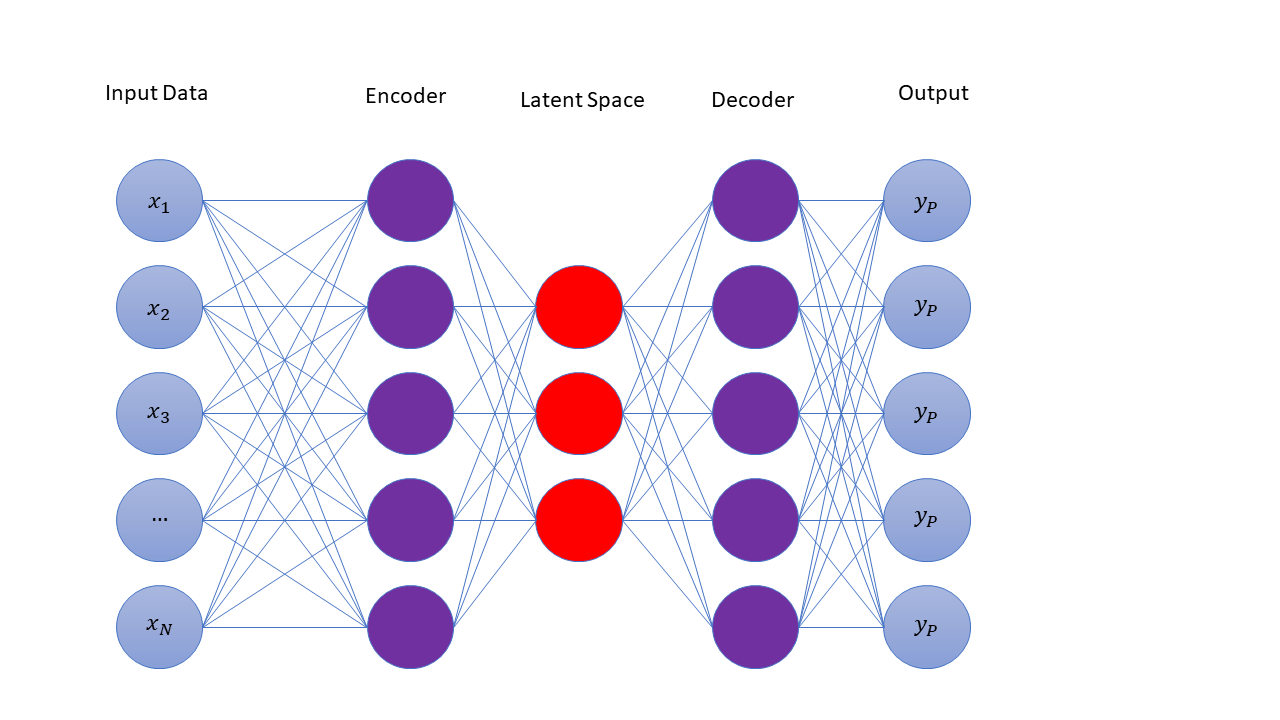
\includegraphics[width=19cm,height=20cm,keepaspectratio]{figures/autoencoder_diagram.png}
    \caption[Simple autoencoder network illustration.]{An autoencoder network composed of two neural networks defined as the encoder 
    and the decoder networks. Here, both networks are represented as fully-connected networks, but could also be any number of other network architectures such \ac{CNN}s and \ac{LSTM} networks. The encoder network takes as input a set of data and compresses the data  
    through a bottleneck called the latent space. The latent space is then given as input to the decoder network which tries to reconstruct the given input $x_1 ... x_N$.}
    \label{fig:autoencoder_diagram}
\end{figure}
\begin{equation}
    l(f(x)) = \sum_k{(f(x)_k - x_k)^2},
\end{equation}
where $f(x)_k$ is the output from the decoder network on the 
kth training/testing sample of the \ac{AE} and $x_k$ is the 
kth training/testing sample. During training, $f(x)_k$ is trained 
to be as similar to $x_k$ as possible in order to minimise 
$l(f(x))$. The lower the value $l(f(x))$ is, the better the network 
is performing. The loss $l(f(x))$ is then backpropagated through 
the network adjusting the weights and biases in order to  
further minimise the loss.

\ac{AE}s can be used across a variety of applications including: 
dimensionality reduction \cite{6910027}, image denoising \cite{NISHIO2017e00393},
feature extraction \cite{7965877} and many others. Although powerful, 
one of the limitations of an \ac{AE} is the way it represents the 
latent space. Within the context of \ac{AE}s as content generators 
the reader would be forgiven for thinking that, if properly trained, 
one could just simply sample from the latent space uniformly 
in order to generate unique content. However, due to the fact 
that the network is not required to distribute learned latent 
space representations during training (features are allowed 
to be encoded anywhere in the latent space), it is not 
guaranteed that latent space samples will be from a 
learned part of the latent space.

%
% Variational autoencoders
%
\subsection{Variational Autoencoders}

A \ac{VAE} (see illustration in 
Fig.\ref{fig:simple_vae}) is nearly identical to an \ac{AE}, except for 
 how the latent space 
is represented and how the loss function is constructed. 
Considering the encoder is given 
a sample MNIST digit image; instead of having the encoder network 
output a single predicted value for each dimension in the 
latent space, we now have it output both a predicted 
mean and standard deviation value describing a Gaussian 
for each dimension. Samples are then drawn from the the 
predicted distributions and given as input the decoder network. 
The decoder network produces estimates trying to reconstruct 
the given input to the encoder network. The loss for 
a \ac{VAE} is also slightly different and is represented 
as 

\begin{figure}
    \centering
    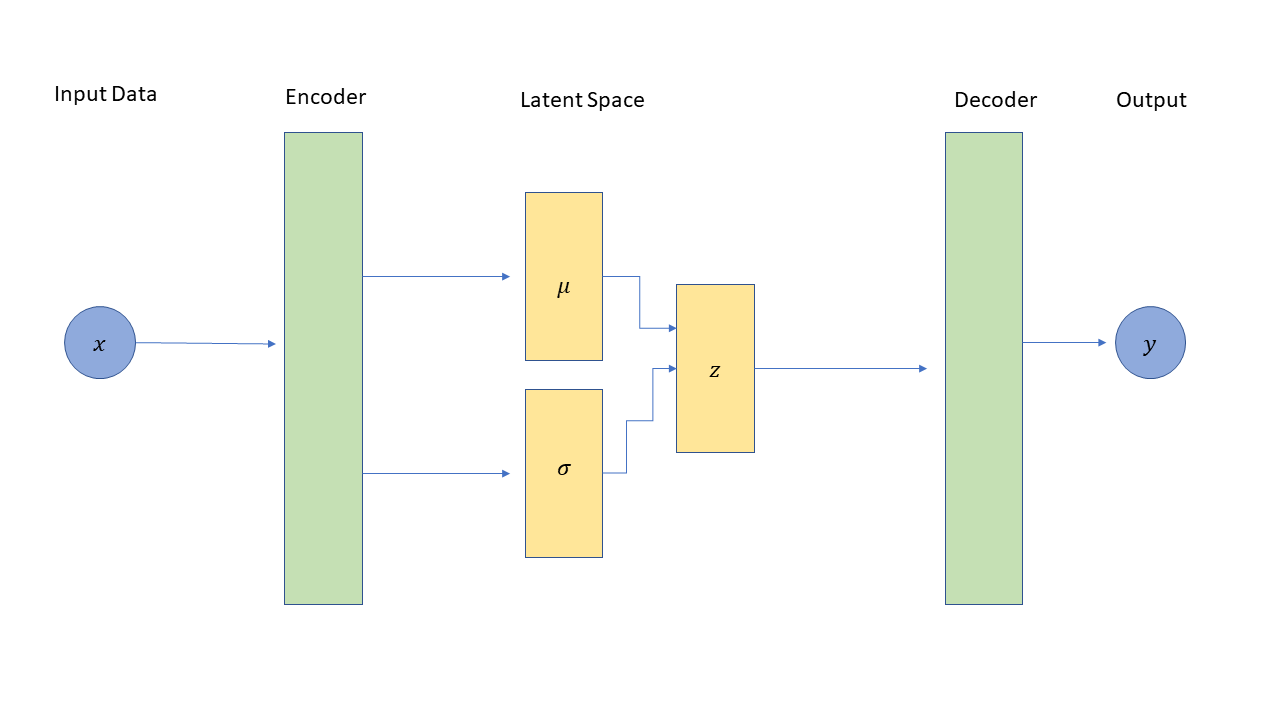
\includegraphics[width=16cm,height=20cm,keepaspectratio]{figures/simple_vae_diagram.png}
    \caption[Simple variational autoencoder network illustration]{A simplified diragram of a variational autoencoder network. The input data $x$ is passed to the encoder neural network which produces predictions on the means $\mu$ and standard deviations $\sigma$ of multi-variate Gaussian distributions describing the latent space. Samples are drawn from the predicted distributions $z$ in order to get samples from the latent space. These latent space samples are then passed to the decoder network which attempts to reconstruct the given input $x$.}
    \label{fig:simple_vae}
\end{figure}
%
\begin{equation}
    l(f(x)) = \sum_k{ (f(x)_k - x_k)^2 + 
    D_{\textrm{KL}}[N(\mu_k, \sigma_k), N(0, 1)]},
\end{equation}
%
where $f(x_k)$ is the predicted output from the decoder, $x_k$
is the given input to the encoder, $D_{\textrm{KL}}$ is the \ac{KL} divergence 
between latent space samples from predicted Gaussians $N(\mu_k, \sigma_k)$ 
and samples from a mean zero unit variant Gaussian 
distribution $N(0,1)$. 

We can derive this loss function by first assuming that we 
want to approximate the optimal latent space posterior 
representation using a neural network. I will be directly following a 
similar derivation done in \cite{1907.08956}. We can define the 
difference between the approximate and the truth as 
%
\begin{equation}
    D_{\textrm{KL}}(q_{\theta}(z|x_k) || p(z|x_k)) = -\int q_{\theta}(z|x_k) \log\left(\frac{p(z|x_k)}{q_{\theta}(z|x_k)}\right) dz,
\end{equation}
%
where $q_{\theta}(z|x_k)$ is the approximate posterior of the 
latent space and $p(z|x_k)$ is the optimal representation. 
We can then substitute Bayes theorem in for the truth 
$p(z|x_k)$ as 
%
\begin{equation}
    D_{\textrm{KL}}(q_{\theta}(z|x_k) || p(z|x_k)) = -\int q_{\theta}(z|x_k) 
    \log\left(\frac{p(x_k|z) p(z)}{q_{\theta}(z|x_k) p(x_k)}\right) dz. 
\end{equation}
%
We now separate out the division using the laws of logarithms and 
distribute the integrand
%
\begin{align}
    D_{\textrm{KL}}(q_{\theta}(z|x_k) || p(z|x_k)) &= -\int q_{\theta}(z|x_k) 
    \left[\log\left(\frac{p(x_k|z) p(z)}{q_{\theta}(z|x_k)}\right) - \log(p(x_k))\right] dz \nonumber \\
    &= -\int q_{\theta}(z|x_k) 
    \log\left(\frac{p(x_k|z) p(z)}{q_{\theta}(z|x_k)}\right) +
    \int q_{\theta}(z|x_k) \log(p(x_k)) dz. 
\end{align}
%
Due to the fact that $q_{\theta}(z|x_k)$ is a probability distribution, 
we can assume that integral of $q_{\theta}(z|x_k)$ is equal to 1, 
further simplifying the equation. We also know that by definition the KL 
divergence must be greater than zero, so we can set the whole 
equation to be greater than or equal to zero
%
\begin{equation}
    -\int q_{\theta}(z|x_k)
    \log\left(\frac{p(x_k|z) p(z)}{q_{\theta}(z|x_k)}\right)dz +
    \int \log(p(x_k)) \geq 0. 
\end{equation}\
%
Since $\log(p(x_k))$ is a constant, we can remove the integrand 
on the right-hand side
%
\begin{equation}
    -\int q_{\theta}(z|x_k)
    \log(\frac{p(x_k|z) p(z)}{q_{\theta}(z|x_k)})dz +
    \log(p(x_k)) \geq 0.
\end{equation}
%
Moving the integral over to the right-hand side we get 
%
\begin{equation}
    \log(p(x_k)) \geq \int q_{\theta}(z|x_k)
    \log\left(\frac{p(x_k|z) p(z)}{q_{\theta}(z|x_k)}\right)dz.\label{eq:lookbackKL}
\end{equation}
%
Applying rules of logarithms yet again, we can now expand 
out the above equation into 
\begin{equation}
    \log(p(x_k)) \geq \int q_{\theta}(z|x_k)
    [\log(p(x_k|z)) + \log(p(z)) - \log(q_{\theta}(z|x_k))] dz.
\end{equation}
We can now recognize that the expression on the right 
is equivalent to the expectation value over the log 
terms given as 
\begin{align}
    \log(p(x_k)) &\geq E_{\sim q_{\theta}(z|x_k)} 
    [\log(p(x_k|z)) + \log(p(z)) - \log(q_{\theta}(z|x_k))] \nonumber \\
    &\geq E_{\sim q_{\theta}(z|x_k)} 
    [\log(p(x_k,z)) - \log(q_{\theta}(z|x_k))].
\end{align}
Taking a small look back to Eq. \ref{eq:lookbackKL}, 
and using the rules of logarithms we can rewrite it as 
\begin{equation}
    \log(p(x_k)) \geq \int q_{\theta}(z|x_k)
    \log\left(\frac{p(z)}{q_{\theta}(z|x_k)}\right)dz + 
    q_{\theta}(z|x_k) \log({p(x_k|z)}) dz
\end{equation}
We can now see clearly that the first expression on the 
right-hand side of the above inequality is equivalent to the 
negative \ac{KL} divergence between our approximate latent space 
representation $q_{\theta}(z|x_k)$ and our prior on 
the latent space $p(z)$
\begin{equation}
    \log(p(x_k)) \geq - D_{\textrm{KL}}(q_{\theta}(z|x_k) || p(z)) + 
    q_{\theta}(z|x_k) \log({p(x_k|z)}) dz. 
\end{equation}
Conveniently, we also see that the right most term on the 
right-hand side of the inequality can be approximated as the 
expectation value of the log probability of the data $x_k$ 
given $z$
\begin{equation}
    \log(p(x_k)) \geq - D_{\textrm{KL}}(q_{\theta}(z|x_k) || p(z)) + 
    E_{\sim q_{\theta}(z|x_k)}[ \log({p(x_k|z)})].\label{eq:vae_loss}
\end{equation}
And there we have it, the loss function for the \ac{VAE}! 
The whole expression to the right of the inequality
is typically denoted as the \ac{ELBO} because it puts a 
lower bound on the log likelihood of the data $log(p(x))$. For 
practical purposes, expectation value on the right can be computed analytically 
by performing the mean squared error between predictions on $x_k$ given 
latent space samples from $q_{\theta}(z|x_k)$ and the true 
$x_k$ values give as input to the encoder. The KL term acts to constrain 
the form of the approximate posterior $\log(p(x_k))$ according to 
a chosen prior on the latent space representation $p(z)$ across the whole input 
parameter space. The KL is essentially a regularization factor which helps 
the model to learn a well-formed latent space and reduce the likelihood 
of overfitting to the training data. $p(z)$ is nominally chosen to be 
represented as a mean zero, unit variant Gaussian distribution. Samples 
are drawn from predicted means and standard deviations from the 
encoder $q_{\theta}(z|x_k)$ and samples are also drawn from a unit variant 
Gaussian representative of the prior $p(z)$. We can then 
analytically compute the KL divergence value. The results from the KL 
and the ELBO calculations are then summed together and the whole term is 
minimized through backpropogation.

%
% reparameterization trick
%
\subsubsection{The Reparameterisation Trick}

First proposed by Kingma et al. in their seminal \ac{VAE} 
paper \cite{1312.6114}, the reparameterization trick acts to 
solve a problem that we now have with the above derived loss 
function for the \ac{VAE}. That problem being that we cannot 
backpropagate the gradient computed with respect to the loss through 
a random node. The random node referred to is the latent space node 
given as input to the decoder which we define as 
\begin{equation}
    z = \mu + \sigma,\label{eq:before_repar} 
\end{equation}
where $z$ are samples from our latent space, $\mu$ are predicted means 
describing multivariate Gaussians and $\sigma$ are predicted standard deviations. 
We can prove that the above equation is nondifferentiable by first rewriting 
the expression as an expectation value
\begin{equation}
    E_{p(z)}[f(z)],
\end{equation}
If we then go to compute the gradient of the expectation value 
(which we would normally do when updating the weights in the 
\ac{VAE}), then we get the following expression

\begin{align}
    \nabla_{\theta} E_{p(z)}[f_{\theta}(z)] &= \nabla_{\theta} \int p(z) f_{\theta}(z) dz \nonumber \\ 
    &= \int p(z) \nabla_{\theta} f_{\theta}(z) dz\nonumber \\
    &= E_{p(z)}[\nabla_{\theta} f_{\theta}(z)],
\end{align}

where it is shown that the gradient of the expectation value 
of $f(z)$ is equivalent to the expectation value of the gradient 
of $f(z)$, which is easily computed since the probability distribution 
is not a function of weights and biases $\theta$. However, if the probability distribution 
were a function of $\theta$, which it is since the latent space is produced 
by the encoder network which is itself a function of weights $\theta$, then 
we see the following happen when taking the gradient of the 
expectation value

\begin{align}
    \nabla_{\theta} E_{p_{\theta}(z)}[f(z)] &= \nabla_{\theta} \int p_{\theta}(z) f_{\theta}(z) dz \nonumber \\
     &= \int \nabla_{\theta}  p_{\theta}(z) f_{\theta}(z) dz \nonumber \\
     &= \int  p_{\theta}(z) \nabla_{\theta} f_{\theta}(z) dz + \int  f_{\theta}(z) dz \nabla_{\theta} p_{\theta}(z) dz \nonumber \\
     &= E_{p_{\theta}(z)}[ \nabla_{\theta} f_{\theta}(z)] + \int  f_{\theta}(z) dz \nabla_{\theta} p_{\theta}(z) dz. \nonumber \\
\end{align}

Although the first summation term is again easily computed, we now are 
left with a particularly intractable integral on the right-hand side.
Monte Carlo methods do allow us to randomly sample from $p_{\theta}(z)$, but 
they do not guarantee that we may take its gradient. 
We are now left with a bit of problem in how we are expected to compute the integral.
However, if we make a small change to Eq. \ref{eq:before_repar} 
by scaling the standard deviation by a deterministic value, we will 
see how this then solves our intractable integral problem. 

If we parameterize this deterministic value as samples drawn 
from a mean zero, unit variant Gaussian distribution 
$\sim N(0, 1)$ which we will denote as 
\begin{equation}
    \epsilon = N(0, 1).
\end{equation}
Then we can rewrite Eq. \ref{eq:before_repar} as 
\begin{equation}
    z = \mu + \sigma \epsilon.
\end{equation}
we'll now simplify the expression to be a function 
$g$ which is parameterized by $\epsilon$ and $x$, 
where $x$ is representative of $\mu$ and $\sigma$
\begin{equation}
    z = g_{\theta}(\epsilon, x).
\end{equation}
rewriting as an expectation value 
\begin{equation}
    E_{p_{\theta}(z)}[f(z^{(i)})] = E_{p(\epsilon)}[
    f(g_{\theta}(\epsilon, x^{(i)}))].
\end{equation}
Taking the gradient with respect to the weights 
and biases of the network $\theta$ we get 
\begin{align}
    \nabla_{\theta} E_{p_{\theta}(z)}[f(z^{(i)})] &= \nabla_{\theta} E_{p(\epsilon)}[
    f(g_{\theta}(\epsilon, x^{(i)}))] \nonumber \\
    &= E_{p(\epsilon)}[ \nabla_{\theta}
    f(g_{\theta}(\epsilon, x^{(i)}))].
\end{align}
where we see that indeed we can take the gradient 
of $f(g_{\theta}(\epsilon, x^{(i)}))$ since 
$g_{\theta}(\epsilon, x^{(i)})$ is differentiable 
with respect to $\theta$. We can now just simply 
randomly Monte Carlo sample in order to analytically 
calculate $\nabla_{\theta} E_{p_{\theta}(z)}[f(z^{(i)})]$.

%
% conditional variational autoencoders
%
\subsection{Conditional Variational Autoencoders}

Through our derivations in the previous sections 
we have now formulated a loss function which can be trained 
to maximize the expected log probability of our 
decoder's prediction, while also regularizing its
model for the latent space to a smooth representation. 
However, there are some minor drawbacks to the \ac{VAE} 
which make it unsuitable for some generative tasks. 

For example, if we wanted to train our \ac{VAE} on 
the fashion MNIST dataset \cite{DBLP:journals/corr/abs-1708-07747}, 
a database of digit images representative of various classes 
of fashion items (shoes, shirts, pants), in order to 
generate new images of fashion items we would run into 
a problem. This problem is most clearly illustrated when 
taking a closer look at Eq. \ref{eq:vae_loss}. In 
Eq. \ref{eq:vae_loss}, it can seen that the encoder 
is solely conditioned on inputs from the training space 
$x_k$, but not on what class/type of image $x_k$ is. Similarly, 
the decoder is solely conditioned on the latent space $z$. In order 
to produce a particular class of input from the decoder, we would have 
to know which part of the latent space each class lives and to then 
draw from the location of the latent space that our class of 
interest resides. Knowledge of class location is infeasible to obtain 
after training because the KL 
divergence term in Eq. \ref{eq:vae_loss} enforces that 
on average across the whole training set that the predicted 
latent space locations are representative 
of a mean zero Gaussian distribution, but does not constrain where 
individual classes of input may reside.

The natural question then arises, is it possible to condition 
the network on classes of interest? It turns out that this is 
possible to do by making a minor update to the 
\ac{VAE} loss in Eq. \ref{eq:vae_loss}
\begin{equation}
    \log(p(x_k)) \geq - D_{\textrm{KL}}(q_{\theta}(z|x_k,c) || p(z,c)) + 
    E_{\sim q_{\theta}(z|x_k,c)}[ \log({p(x_k|z,c)})].
\end{equation}
Here, we now condition the encoder $q_{\theta}(z|x_k,c)$ on both 
the training images $x_k$ and the class of said images $c$ (see Fig.\ref{fig:simple_cvae}). In the decoder 
$p(x_k|z,c)$ we condition on samples from the latent space $z$ and the 
class $c$. For classification purposes, the class is usually 
parameterized as a single scalar number which is appended to the input to 
the encoder and decoder networks. Now, if we wanted to use the decoder 
as a fashion image generator, we would only simply need to draw a 
random sample from the latent space, choose a class number, and then 
feed both as inputs to the decoder network. 

\begin{figure}
    \centering
    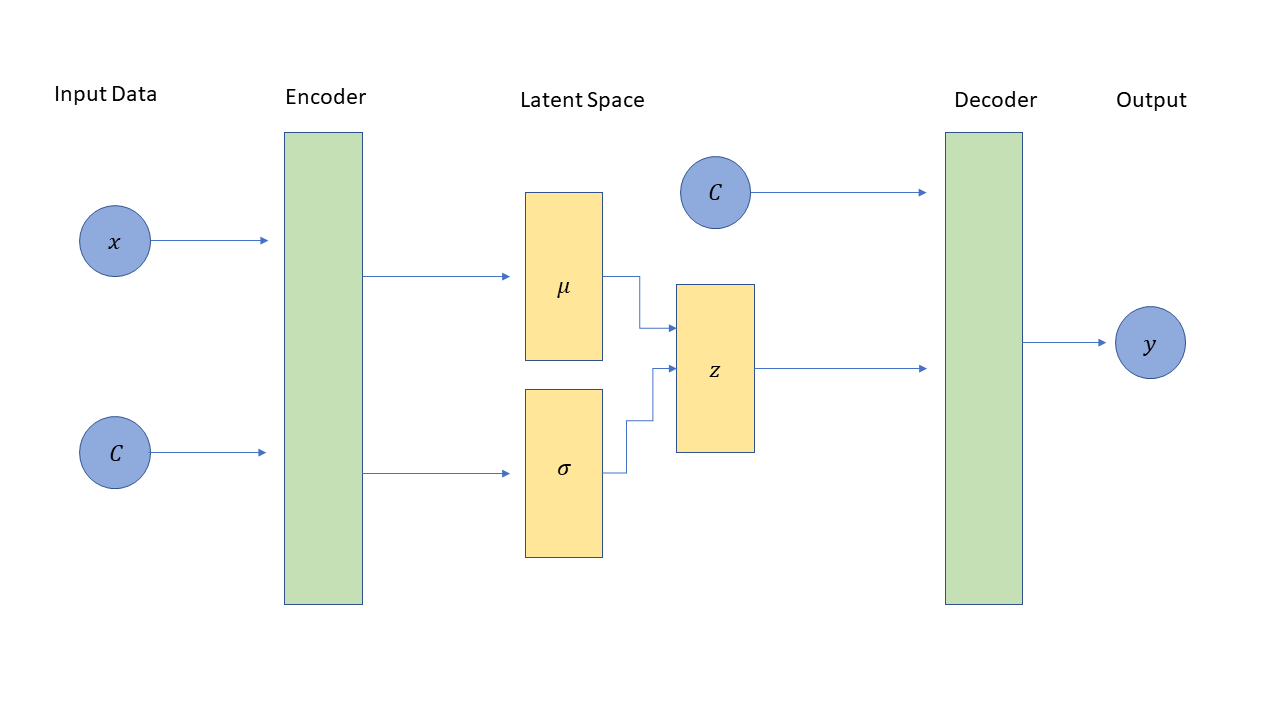
\includegraphics[width=16cm,height=20cm,keepaspectratio]{figures/simple_cvae_diagram.png}
    \caption[Simple conditional variational autoencoder illustration.]{A simple \ac{CVAE} diagram consisting of an encoder and decoder network. $x$ data is given as input to the encoder and latent space samples are given as input to the decoder as was the case with the \ac{VAE} diagram in Fig.\ref{fig:simple_vae}. However, now we additionally condition the encoder on the class of $x$ by appending the class label in numerical form to $x$. We also condition the decoder on class $c$ by appending it to the latent space samples $z$.}
    \label{fig:simple_cvae}
\end{figure}

\section{Summary}

In this chapter we introduced the concept of machine learning 
starting from one of the simplest neural networks, a perceptron. We 
then built on perceptrons discussing how perceptrons can be strung 
together to make a neural network layer, and from there layers 
can be stacked to form a multi-layer deep fully-connected neural network. 
I also provided some best practices on hyperparameter optimisation and 
training procedures. We introduce the concept of both a \ac{CNN} 
and a \ac{CVAE}, two of the networks primarily used in this author's 
thesis work. In the following chapter (Ch.~\ref{ch:chap_3}), we will 
discuss how \ac{ML} is being applied across a variety of domains in 
\ac{GW} astronomy to great success. 